\documentclass[]{article}
\usepackage{lmodern}
\usepackage{amssymb,amsmath}
\usepackage{ifxetex,ifluatex}
\usepackage{fixltx2e} % provides \textsubscript
\ifnum 0\ifxetex 1\fi\ifluatex 1\fi=0 % if pdftex
  \usepackage[T1]{fontenc}
  \usepackage[utf8]{inputenc}
\else % if luatex or xelatex
  \ifxetex
    \usepackage{mathspec}
    \usepackage{xltxtra,xunicode}
  \else
    \usepackage{fontspec}
  \fi
  \defaultfontfeatures{Mapping=tex-text,Scale=MatchLowercase}
  \newcommand{\euro}{€}
\fi
% use upquote if available, for straight quotes in verbatim environments
\IfFileExists{upquote.sty}{\usepackage{upquote}}{}
% use microtype if available
\IfFileExists{microtype.sty}{%
\usepackage{microtype}
\UseMicrotypeSet[protrusion]{basicmath} % disable protrusion for tt fonts
}{}
\usepackage[margin=1in]{geometry}
\usepackage{longtable,booktabs}
\usepackage{graphicx}
\makeatletter
\def\maxwidth{\ifdim\Gin@nat@width>\linewidth\linewidth\else\Gin@nat@width\fi}
\def\maxheight{\ifdim\Gin@nat@height>\textheight\textheight\else\Gin@nat@height\fi}
\makeatother
% Scale images if necessary, so that they will not overflow the page
% margins by default, and it is still possible to overwrite the defaults
% using explicit options in \includegraphics[width, height, ...]{}
\setkeys{Gin}{width=\maxwidth,height=\maxheight,keepaspectratio}
\ifxetex
  \usepackage[setpagesize=false, % page size defined by xetex
              unicode=false, % unicode breaks when used with xetex
              xetex]{hyperref}
\else
  \usepackage[unicode=true]{hyperref}
\fi
\hypersetup{breaklinks=true,
            bookmarks=true,
            pdfauthor={Fauzy bin Che Yayah},
            pdftitle={Automated Text Data Processing Techniques on Trouble Ticket for Enhancing Resolution Knowledge in Bigdata Perspective},
            colorlinks=true,
            citecolor=blue,
            urlcolor=blue,
            linkcolor=magenta,
            pdfborder={0 0 0}}
\urlstyle{same}  % don't use monospace font for urls
\setlength{\parindent}{0pt}
\setlength{\parskip}{6pt plus 2pt minus 1pt}
\setlength{\emergencystretch}{3em}  % prevent overfull lines
\setcounter{secnumdepth}{5}

%%% Use protect on footnotes to avoid problems with footnotes in titles
\let\rmarkdownfootnote\footnote%
\def\footnote{\protect\rmarkdownfootnote}

%%% Change title format to be more compact
\usepackage{titling}

% Create subtitle command for use in maketitle
\newcommand{\subtitle}[1]{
  \posttitle{
    \begin{center}\large#1\end{center}
    }
}

\setlength{\droptitle}{-2em}
  \title{Automated Text Data Processing Techniques on Trouble Ticket for
Enhancing Resolution Knowledge in Bigdata Perspective}
  \pretitle{\vspace{\droptitle}\centering\huge}
  \posttitle{\par}
  \author{Fauzy bin Che Yayah}
  \preauthor{\centering\large\emph}
  \postauthor{\par}
  \predate{\centering\large\emph}
  \postdate{\par}
  \date{November 11, 2015}



\begin{document}

\maketitle


\section{Abstract}\label{abstract}

\emph{Trouble ticket system is always includes very rich data, but how
to data-mining from is very challenging task.In this paper we apply the
technique of data processing for the ease for the next stage of
classification and prediction.On the other hand , we applied new
technology of data mining by combining with the Bigdata elements for
faster and achievable results.}

\section{Keywords}\label{keywords}

Data processing ; Hadoop ; Trouble tickets

\section{Introduction}\label{introduction}

The trouble ticket system for telecommunication industries produced
several thousand of records everyday. These records provide rich,
accurate and complete for the system diagnostics and enhancing the
customer experience by solving the problems. The live records stored
inside the database of all levels of servers and replicated into the
Enterprise Data Warehouse (EDWH) for data staging and shared among the
departments via the credential and permission for different points of
usage or use case. The data are coordinated and conserved for at least
for five years minimum, which is enough for the analytics and data
discovery purpose. The remaining more than five years of data will not
be discarded and the archiving process will be applied for future
reference. Because of the EDWH is optimized for storage, any heavily
queries for analytics purpose in the system is not recommended which
this activity will jeopardize the overall system performance.

\section{Trouble ticket system (TTS)}\label{trouble-ticket-system-tts}

\subsection{Introduction of TTS}\label{introduction-of-tts}

The trouble ticket system is considered as an assistant software which
implements the Decision Support System (DSS) that manage and maintain
lists of issues recorded by the customer support call center. The system
contains a knowledge based containing the vital information for each
subscribed customer, common resolution for most of the problems, and
other such data. The ticket is the details of particular problem which
contains the ticket status and other relevant data.

\begin{figure}[htbp]
\centering
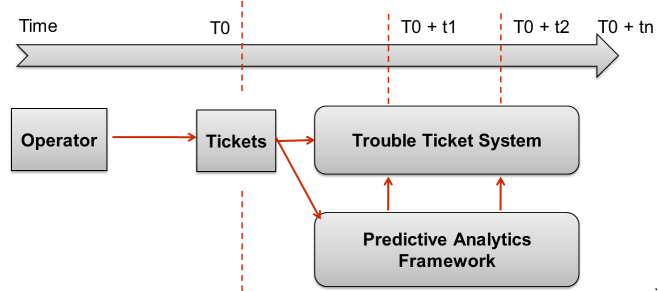
\includegraphics{tts.png}
\caption{Trouble ticket system with predictive analytics framework}
\end{figure}

\subsection{Basic structure of trouble ticket
data}\label{basic-structure-of-trouble-ticket-data}

The dataset of customer trouble ticket mainly comes from the trouble
ticket system (TTS). The data set, then distributed into different
levels of staging servers and other type database system at different
levels of credential. The table below is a list of some fields from the
trouble ticket table which mapped from the CTTS database :-

\begin{longtable}[c]{@{}lll@{}}
\toprule
Column Name & Column Type & Notes\tabularnewline
\midrule
\endhead
id & String & Generated ID by the system\tabularnewline
created\_dt & DateTime & Date of the trouble ticket
creation\tabularnewline
closed\_dt & DateTime & Date of the trouble ticket closed\tabularnewline
symp\_err & String & Symptom error detected\tabularnewline
cause\_cat & String & Category Code define by the system\tabularnewline
cause\_code & String & Cause Code define by the system\tabularnewline
res\_code & String & Resolution Code define\tabularnewline
desc & Text & Detail textual information such as\tabularnewline
& & customer information, session status,\tabularnewline
& & system status, network status , etc.\tabularnewline
& & Cause Code define by the system\tabularnewline
acc\_name & String & Name of the customer\tabularnewline
acc\_num & String & Account number of the customer\tabularnewline
package & String & Main package subscribed by the
customers\tabularnewline
zone & String & Product affected zone\tabularnewline
\ldots{}. & \ldots{}. & \ldots{}.\tabularnewline
\bottomrule
\end{longtable}

\newpage

In summary , this table below is the sample of TTS records :-

\begin{longtable}[c]{@{}lll@{}}
\toprule
Column Type & Example & Field Name\tabularnewline
\midrule
\endhead
Integer & {[}1001{]} , {[}1002{]} , {[}1003{]} & ID\tabularnewline
DateTime & {[}2012-09-05 19:39:01.0{]},{[}2012-09-05 19:45:39.0{]} &
created\_dt\tabularnewline
Text & \emph{``Troubleshooting Step: -check outages -check account
status''} & desc\tabularnewline
String & {[}Performance{]} , {[}Failure{]}, {[}Open{]}, {[}Closed{]} &
symp\_err\tabularnewline
\ldots{}. & \ldots{}. & \ldots{}.\tabularnewline
\bottomrule
\end{longtable}

We identify the structure inside the TTS (\emph{desc}) contains a free
text form inside the description field. This is in need for search and
analyze inside it. The data need to transform into something that can
have a better understanding and more effective representation. A TTS
description is fill-up by capturing from the customer call center or by
the technician from the two major sources such as email and subsequent
call from the customer.Thus, most of the data is not explicitly
structured, it is also highly noisy (e.g, inconsistent formatting) and
also very heterogenous (e.g., multiple language, such as Bahasa Melayu
or English, system generated data, specific telecommunication term ,
abbreviation , acronyms and jargons),making it hard to analyze and
search information from the raw data. We introduced an approach for
automatically search for specific knowledge or topics from the
collection of the free from text section (desc) inside the TTS.

\section{Methods}\label{methods}

Our elegant methodology automatically structuring free-from heterogenous
textual data helps to identify the structural pattern specific pattern
known to the call center of technician which helps them to speed up the
tedious work manually searching and understanding the relevant data
inside it. Below is the workflow for this methodology :-

\begin{itemize}
\itemsep1pt\parskip0pt\parsep0pt
\item
  Acquiring with basic filtering TTS dataset from EDWH into Hadoop using
  Sqoop
\item
  Applying index number for TTS dataset inside Hive
\item
  Second filtering TTS dataset
\item
  Create a Document Term Matrix (DTM)
\item
  Remove Sparse Terms
\item
  Vectorize TTS (VTTS)
\item
  VTTS and DTM
\item
  Training
\item
  Testing
\item
  Prediction
\end{itemize}

\subsection{Acquiring with basic filtering TTS dataset from EDWH into
Hadoop using
Sqoop}\label{acquiring-with-basic-filtering-tts-dataset-from-edwh-into-hadoop-using-sqoop}

To acquire TTS dataset from the EDWH we need special operation using
\emph{Sqoop} components inside Hadoop into Hive compatible format.
Hadoop is an open-source software framework for storing data and running
applications on clusters of commodity hardware. Hive is a data warehouse
infrastructure built on top of Hadoop for providing data summarization,
query, and analysis.Sqoop is a tool designed to transfer data between
Hadoop and relational database servers.

\begin{figure}[htbp]
\centering
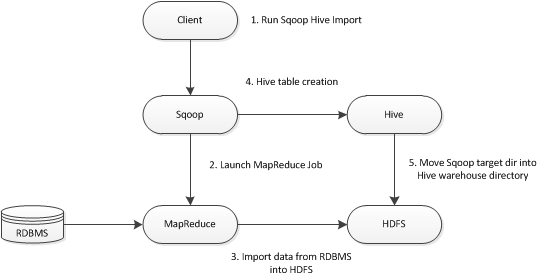
\includegraphics{hivesqoophadoop.png}
\caption{Hadoop - Sqoop - Hive Operation}
\end{figure}

\newpage

Sqoop basic syntax for importing dataset from TTS as follows :-

\begin{verbatim}
sqoop import --connect jdbc:[rdbms driver]:@[ip_address]:[port]/[db_name] 
--username [username] --password [password]  --target-dir [temp_target]  --verbose 
-e "select [field[1:n],REGEXP_REPLACE([desc_field_name],
'[^a-zA-Z0-9\\:\\@\\/\\#\\-]', ' ') " --m 1 --hive-table 
[dbname_in_hdfs][tablename_inhdfs] --hive-import
--append --fields-terminated-by '\001'  
--lines-terminated-by '\n' --hive-delims-replacement '';
\end{verbatim}

Description of the syntax above as follows :-

\begin{longtable}[c]{@{}ll@{}}
\toprule
Syntax & Description\tabularnewline
\midrule
\endhead
sqoop import & Import a table from a database to HDFS\tabularnewline
--connect jdbc:{[}rdbms driver{]} & Specify JDBC connect
string\tabularnewline
{[}ip\_address{]}:{[}port{]}/{[}db\_name{]} & Provides ip address , port
no and rdbms database name\tabularnewline
--username {[}username{]} & Provides the username\tabularnewline
--password {[}password{]} & Provides the password\tabularnewline
--target-dir {[}temp\_target{]} & Specify the target path for the output
of the merge job\tabularnewline
--verbose & Print information while execute\tabularnewline
-e & specified query statement\tabularnewline
\emph{select} & statement returns a result set of records from one or
more tables\tabularnewline
{[}field{[}1:n{]} &\tabularnewline
REGEXP\_REPLACE({[}desc\_field\_name{]},) & search a string for a
regular expression pattern\tabularnewline
`{[}\^{}a-zA-Z0-9\textbackslash{}\textbackslash{}:\textbackslash{}\textbackslash{}@\textbackslash{}\textbackslash{}/\textbackslash{}\textbackslash{}\#\textbackslash{}\textbackslash{}-{]}',
`') & remove all special characters and numbers\tabularnewline
{[}-m 1{]} & Use n map tasks to import in parallel\tabularnewline
{[}--hive-table & Sets the table name to use when importing to
Hive\tabularnewline
{[}{[}dbname\_in\_hdfs{]} & Sets the db name in Hive/HDFS\tabularnewline
{[}tablename\_inhdfs{]} & Sets the db name in Hive/HDFS\tabularnewline
--hive-import & Import tables into Hive format\tabularnewline
--append & Append data to an existing dataset in HDFS\tabularnewline
--fields-terminated-by `\textbackslash{}001' & Sets the field separator
character\tabularnewline
--lines-terminated-by `\textbackslash{}n' & Sets the end-of-line
character\tabularnewline
--hive-delims-replacement '' & Replace delimiter from string fields with
user defined string\tabularnewline
\bottomrule
\end{longtable}

To make, it is safe to resides into the Hive table, any special
character set by \texttt{REGEXP\_REPLACE} found during acquiring the
dataset will be replaced with default delimiter \texttt{NULL} or empty
char. this can be achieved by applying the
\texttt{-\/-hive-delims-replacement \textquotesingle{}\textquotesingle{}}
and \texttt{REGEXP\_REPLACE}
\texttt{{[}\^{}a-zA-Z0-9\textbackslash{}\textbackslash{}:\textbackslash{}\textbackslash{}@\textbackslash{}\textbackslash{}/\textbackslash{}\textbackslash{}\#\textbackslash{}\textbackslash{}-{]}}
inside the command line while sqoop is executed. The comparison results
show below :-

\begin{longtable}[c]{@{}l@{}}
\toprule
Original - (desc) structure\tabularnewline
\midrule
\endhead
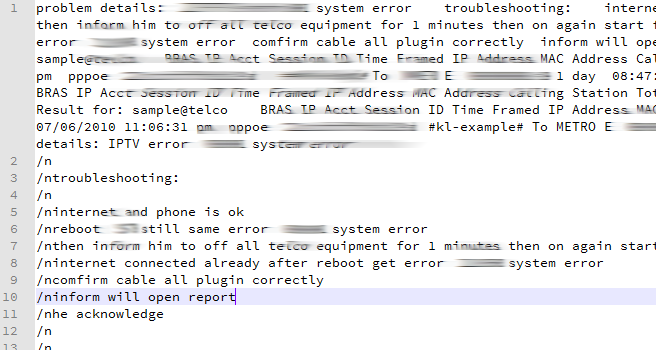
\includegraphics{before.png}\tabularnewline
\bottomrule
\end{longtable}

\begin{longtable}[c]{@{}l@{}}
\toprule
Filtered - (desc) structure after applying REGEXP\_REPLACE during
\texttt{Sqoop} operation\tabularnewline
\midrule
\endhead
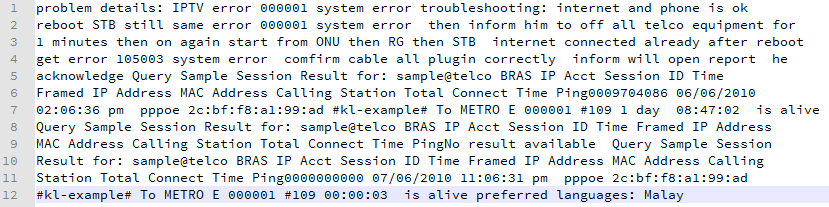
\includegraphics{after.png}\tabularnewline
\bottomrule
\end{longtable}

\subsection{Applying index number for TTS dataset inside
Hive}\label{applying-index-number-for-tts-dataset-inside-hive}

Basic sqoop dataset creation in Hadoop

\subsection{Second filtering TTS
dataset}\label{second-filtering-tts-dataset}

Basic sqoop dataset creation in Hadoop

\section{Results}\label{results}

Note that the \texttt{echo = FALSE} parameter was added to the code
chunk to prevent printing of the R code that generated the plot.

\section{Discussion}\label{discussion}

Note that the \texttt{echo = FALSE} parameter was added to the code
chunk to prevent printing of the R code that generated the plot.

\section{Acknowledgments}\label{acknowledgments}

Note that the \texttt{echo = FALSE} parameter was added to the code
chunk to prevent printing of the R code that generated the plot.

\section{References}\label{references}

Note that the \texttt{echo = FALSE} parameter was added to the code
chunk to prevent printing of the R code that generated the plot.

\end{document}
